\documentclass[../main.tex]{subfiles}

\graphicspath{{../images/}}

\begin{document}
\pagestyle{fancy}
\lhead{Homework 8}
\chead{Junseo Shin}
\rhead{PHYS 421}

%  HW 5: 5.1, 5.3, 5.4, 5.5, 5.6, 5.11
\begin{center}
    \section*{Homework 8}
    % add to toc
    \addcontentsline{toc}{section}{Homework 8}
\end{center}

\paragraph{5.1} % fig hw8_1.png
\begin{figure*}[ht]
    \centering
    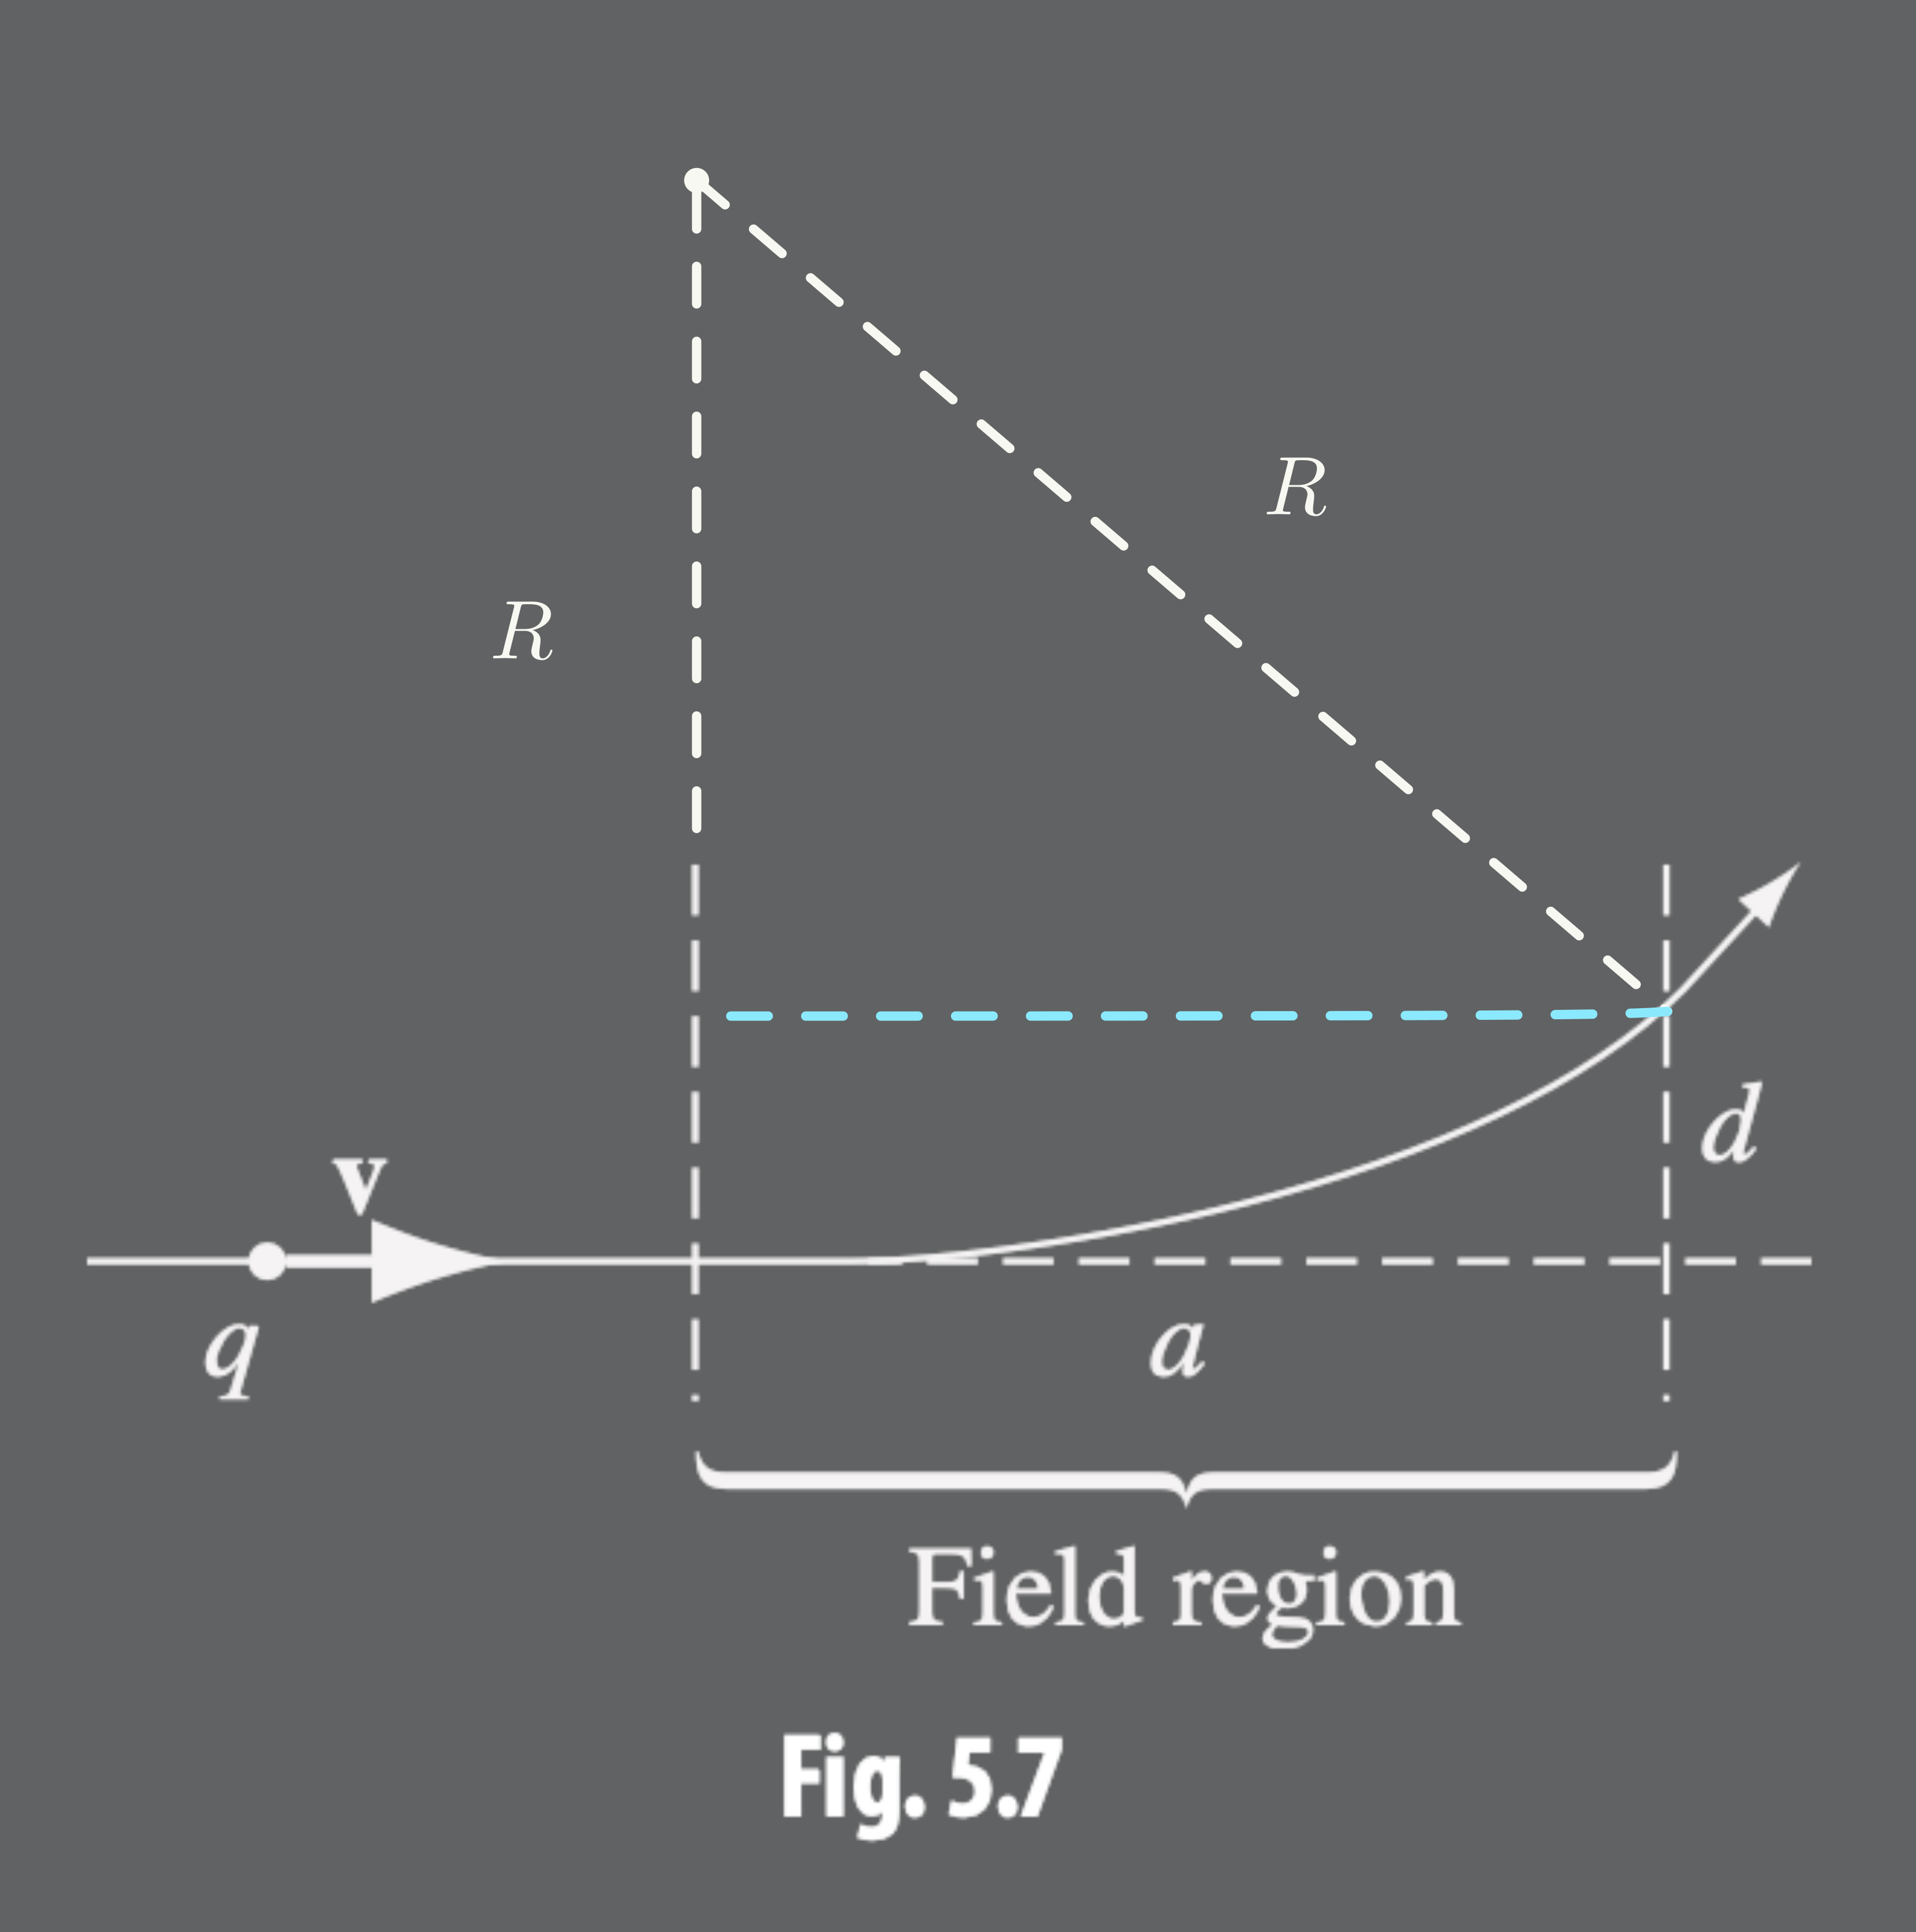
\includegraphics[width=0.5\textwidth]{hw8_1.png}
    \caption{Extended geometry of particle path}
    \label{fig:hw8_1}
\end{figure*}
From Griffiths, the momentum of the particle is given by the cyclotron formula
\begin{align*}\tag{5.3}\label{eq:5.3}
    p = qBR
\end{align*}
So from Fig. \ref{fig:hw8_1}, the radius of the path is given by
\begin{align*}
    R^2 &= (R - d)^2 + a^2 \\
    R^2 &= R^2 - 2Rd + d^2 + a^2 \\
    \implies R &= \frac{d^2 + a^2}{2d}
\end{align*}
Thus
\begin{align*}
    \boxed{
        p = qB\frac{d^2 + a^2}{2d} 
    }
\end{align*}

\newpage
\paragraph{5.3}
\begin{enumerate}
    \item [(a)] Adjusting the beam for zero deflection means that the Lorentz force is zero:
    \begin{align*}
        \vb F = q(\vb E + \vb v \times \vb B) = 0 \\
        \implies \vb E = -\vb v \times \vb B
    \end{align*}
    or in terms of the magnitude 
    \begin{align*}
        \boxed{
            v = \frac{E}{B}
        }
    \end{align*}
    \item [(b)] Using \ref{eq:5.3} and the result from (a),
    \begin{align*}
        p = mv = qBR \\
        \implies \frac{q}{m} = \frac{v}{BR} = \boxed{\frac{E}{B^2R}}
    \end{align*}
\end{enumerate}

\newpage
\paragraph{5.4} 
\begin{figure*}[ht]
    \centering
    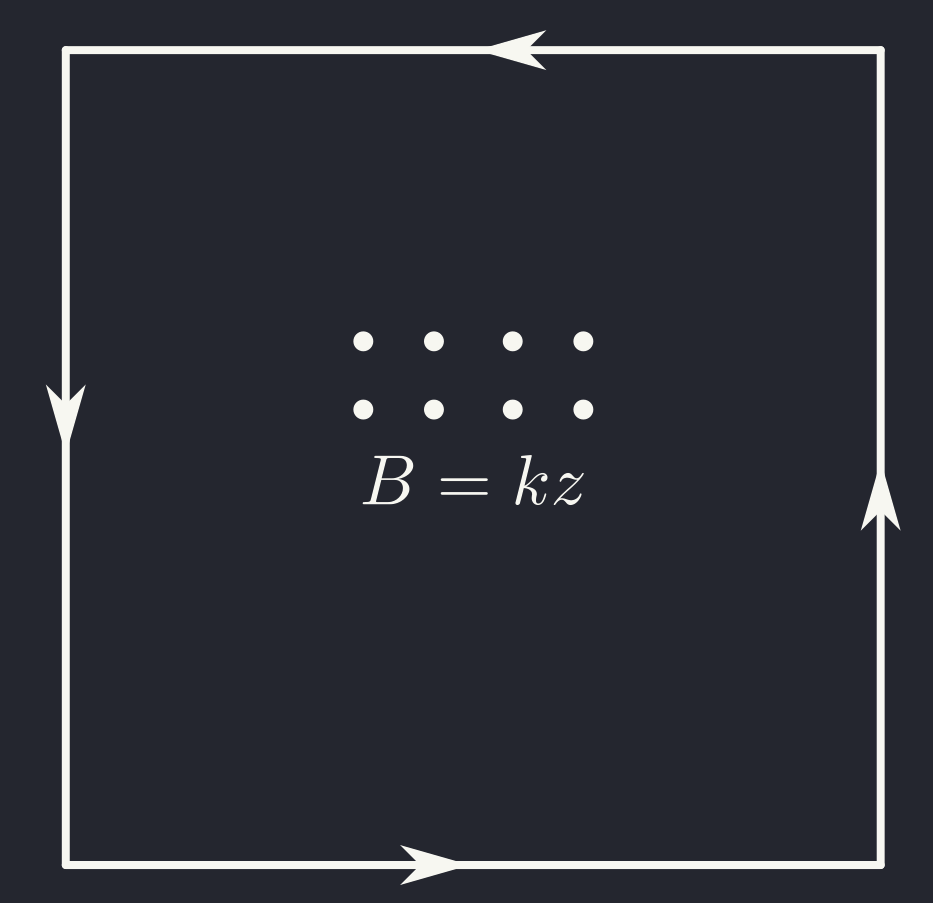
\includegraphics[width=0.3\textwidth]{hw8_2.png}
    \caption{View from $yz$ plane: Magnetic field points out of the page, on the}
    \label{fig:hw8_2}
\end{figure*}
Given the magnetic field
\begin{align*}
    \vb B = kz \vu x
\end{align*}
Using RHR:
\begin{itemize}
    \item The left side of the loop has a force pointing to the left $(-\vu y)$ which cancels out with the 
    \item Right side of the loop with force pointing to the right $(\vu y)$
    \item The top ($z = a/2$) and bottom ($z = -a/2$) side of the loop have forces pointing in the same direction $(\vu z)$
\end{itemize}
So the two forces are
\begin{align*}
    F_\text{top} &= 2 I Ba = I (k a/2) a = \frac{1}{2} I k a^2, \quad F_\text{ bottom} = -\frac{1}{2} I k a^2
\end{align*}
and since they are in the same direction, the net force is
\begin{align*}
    \vb F = I k a^2 \vu z
\end{align*}

\newpage
\paragraph{5.5} For a wire of radius $a$
\begin{enumerate}
    \item [(a)] If the current is uniformly distributed over the surface, the current density is
    \begin{align*}
        K = \dv{I}{dl_\perp} = \frac{I}{2\pi a}
    \end{align*}
    since the width of the ribbon $\dd{l_\perp}$ is the circumference of the wire cross-section.
    \item [(b)] If the volume current density is inversely proportional to the distance from the axis,
    we can use the result from (a):
    \begin{align*}
        J(s) = \frac{k}{s}
    \end{align*}
    and integrating to find $k$:
    \begin{align*}
        I &= \int J(s) \dd{A} = k \int \frac{1}{s} (s \dd{s} \dd{\phi}) \\
        &= k (2\pi) \int_0^a \dd{s} = 2\pi k a \\
        \implies k &= \frac{I}{2\pi a}
    \end{align*}
    or the same result as (a). Thus
    \begin{align*}
        \boxed{
            J(s) = \frac{I}{2\pi a s}
        }
    \end{align*}
\end{enumerate}

\newpage
\paragraph{5.6}
\begin{enumerate}
    \item [(a)] A phonograph with static electricity $\sigma$ rotating at $\omega$.
    The surface current density $K$ at a distance $r$ from the center is (using $v = r\omega$)
    \begin{align*}
        K = \sigma v = \boxed{\sigma r \omega}
    \end{align*}
    \item [(b)] A uniform sphere of radius $R$ with charge $Q$ spins around the $z$ axis at a constnat angular velocity $\omega$.
    The volume current density $\vb J$ at any point in the sphere is (using $v = r\omega \sin\phi$)
    \begin{align*}
        \vb J = \rho \vb v = \rho r \omega \sin\phi \vu \phi
    \end{align*}
    where $\rho = \frac{Q}{4\pi R^3/3}$ is the charge per volume of the sphere, so 
    \begin{align*}
        \boxed{
            \vb J = \frac{Q}{4\pi R^3} r \omega \sin\phi \vu \phi
        }
    \end{align*}
\end{enumerate}

\newpage
\paragraph{5.11} For a tightly wound solenoid with $n$ turns per unit length and radius $a$, we start with a single loop (From Griffiths Example 5.6)
\begin{align*}
    B_\text{loop} &= \frac{\mu_0 I}{4\pi} \int \frac{\dd{l'}}{\scriptr^2} \cos\theta = \frac{\mu_0 I}{4\pi} \qt(\frac{\cos\theta}{\scriptr}) 2 \pi a \\
    &= \frac{\mu_0 I}{2} \frac{a^2}{(a^2 + z^2)^{3/2}}
\end{align*}
so for $n$ turns per unit length we multiply by $n$ and integrate over the length of the solenoid
\begin{align*}
    B &= \frac{\mu_0 n I}{2} \int \frac{a^2}{(a^2 + z^2)^{3/2}} \dd{z}
\end{align*}
Using $\tan\theta = a/z \implies z = a / \tan\theta$ and $\dd{z} = - \frac{a}{\sin^2\theta}\dd{\theta}$, the integral becomes
\begin{align*}
    \int \frac{a^2}{(a^2 + (a/\tan\theta)^2)^{3/2}} \qt(-\frac{a}{\sin^2\theta}) \dd{\theta}) &= -\int \frac{a^2}{(a^2)^{3/2} \qt(1 + \frac{\cos^2\theta}{\sin^2\theta})^{3/2}} \qt(\frac{a}{\sin^2\theta}) \dd{\theta} \\
    &= -\int \frac{1}{\frac{1}{(\sin^2\theta)^{3/2}} (\sin^2\theta + \cos^2\theta)^{3/2} \sin^2\theta} \dd{\theta} \\
    &= - \int \frac{\sin^3\theta}{\sin^2\theta} \dd{\theta} \\
    &= - \int \sin\theta \dd{\theta} = \cos\theta \eval_{\theta_1}^{\theta_2} = \cos\theta_2 - \cos\theta_1
\end{align*}
So
\begin{align*}
    \boxed{
        B = \frac{\mu_0 n I}{2} (\cos\theta_2 - \cos\theta_1)
    }
\end{align*}
\begin{figure*}[ht]
    \centering
    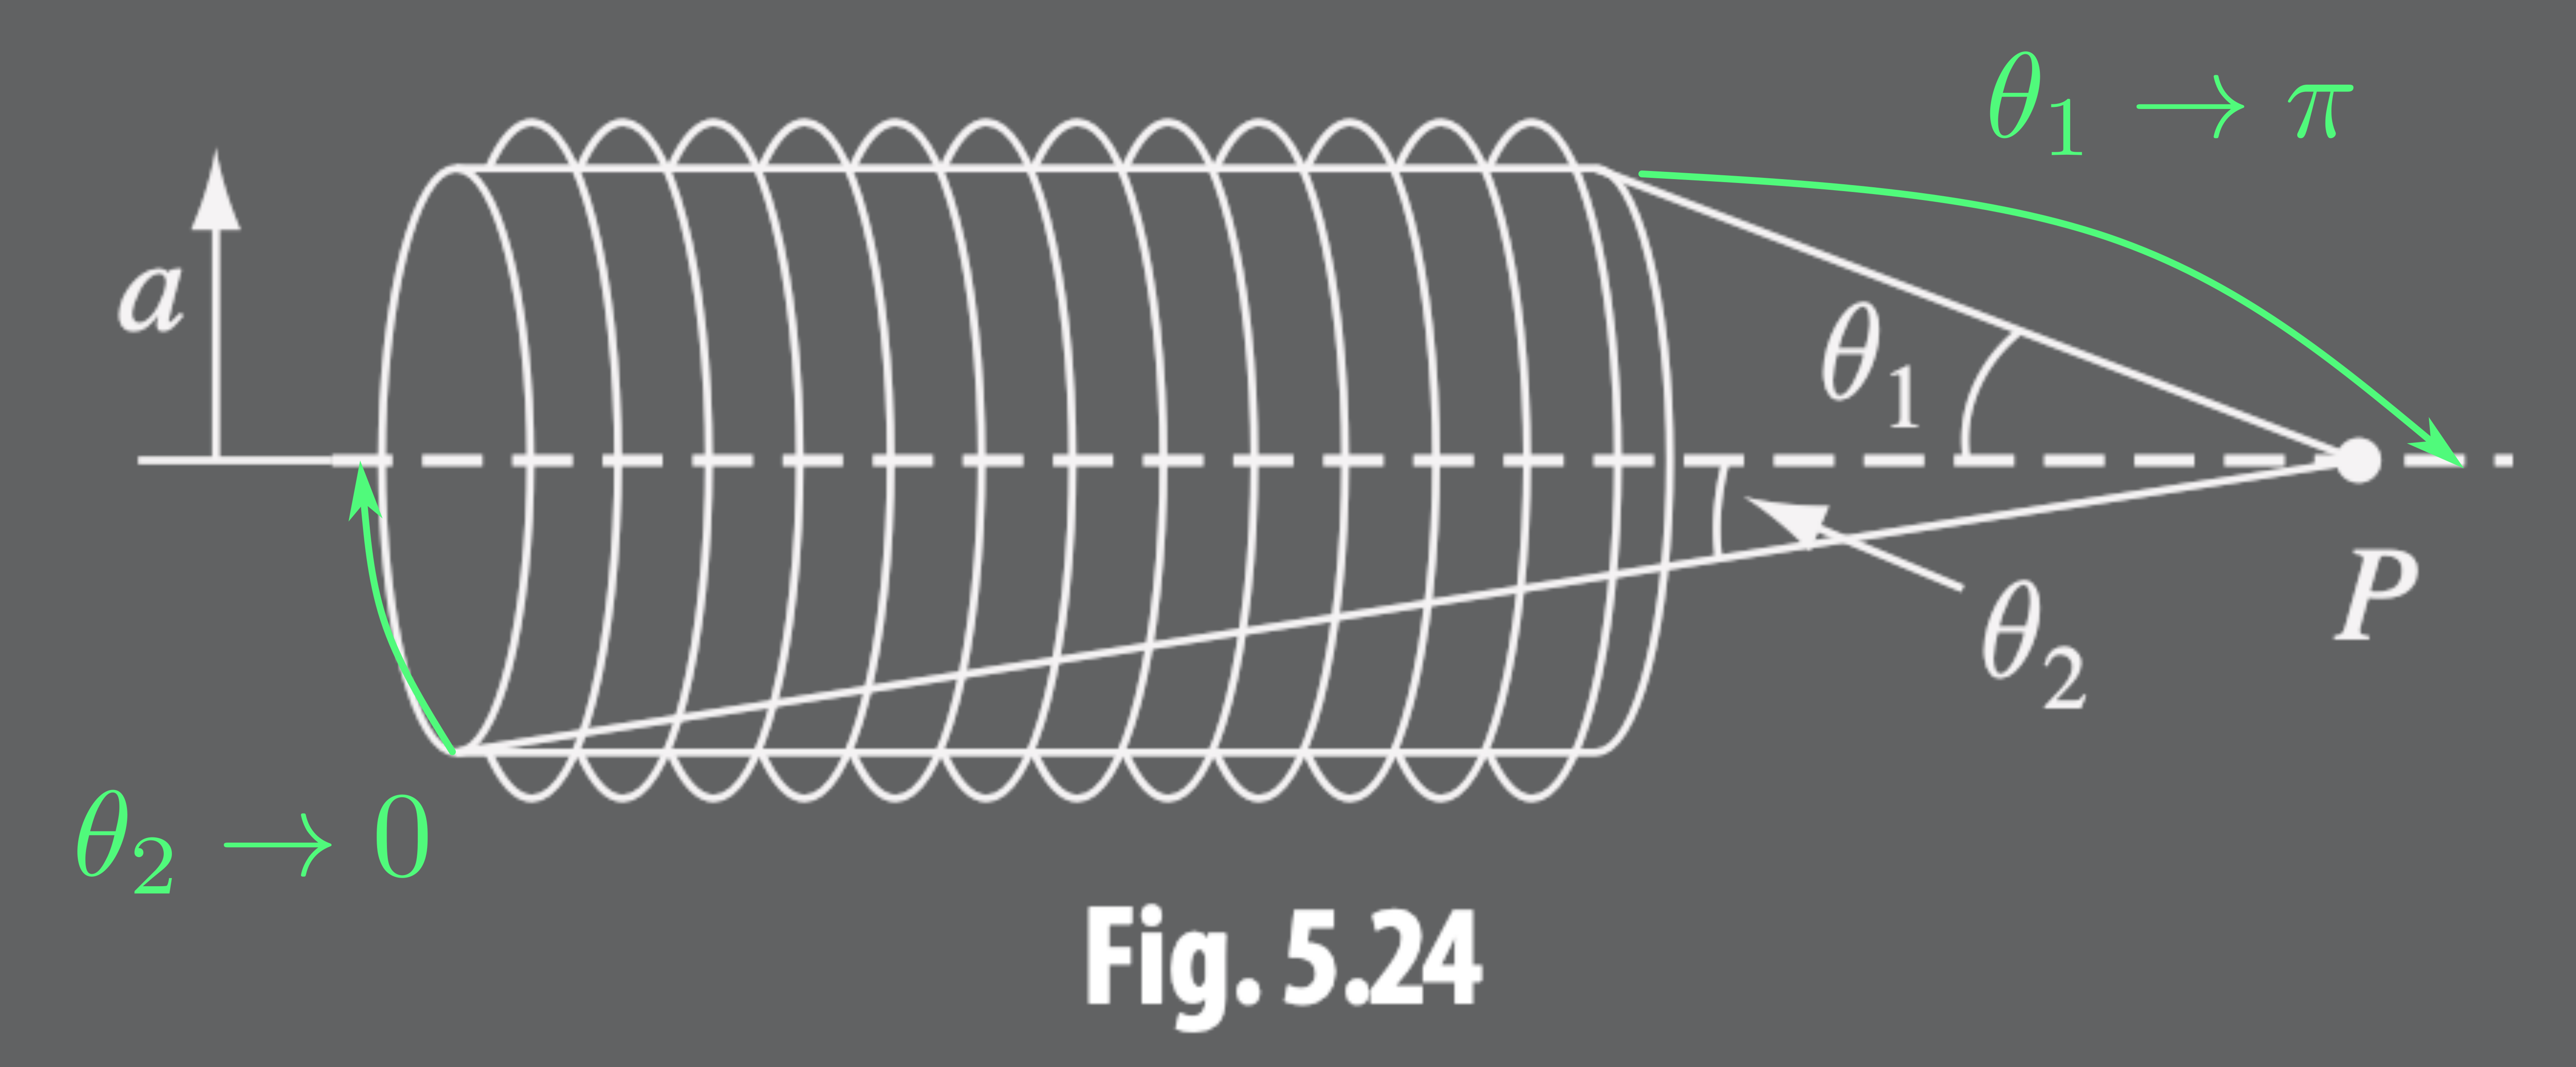
\includegraphics[width=0.5\textwidth]{hw8_3.png}
    \caption{As solenoid becomes infinitely long, $\theta_2 \to 0$ and $\theta_1 \to \pi$}
    \label{fig:hw8_3}
\end{figure*}

As the solenoid becomes infinitely long (Fig.\ref{fig:hw8_3}), then $\theta_2 \to 0$ and $\theta_1 \to \pi$ so
\begin{align*}
    B = \frac{\mu_0 n I}{2} (1 - (-1)) = \boxed{\mu_0 n I}
\end{align*}
\end{document}